\begin{wrapfigure}{r}{0.35\textwidth}
\vspace{-1.0cm}
  \begin{center}
    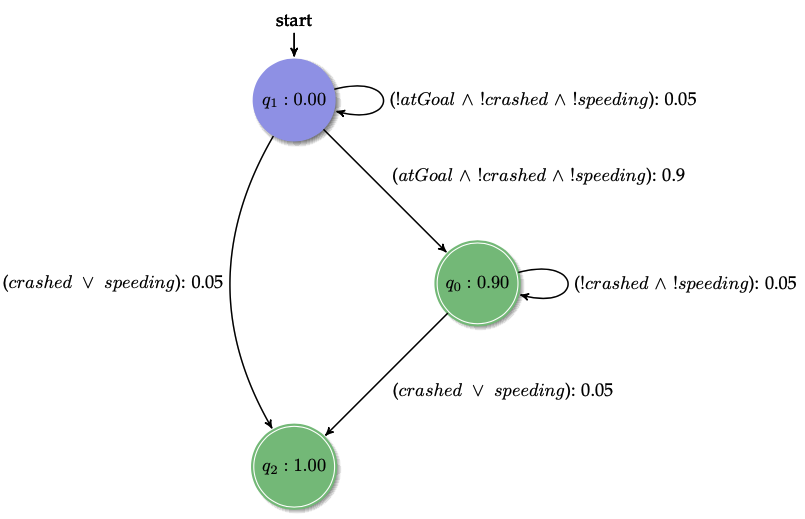
\includegraphics[width=0.35\textwidth]{Figures/PDFA.png}
  \end{center}
  \caption{An example of a probabilistic deterministic finite automaton (PDFA) specification for one of my toy autonomous driving scenarios.}
  \label{fig: driving_pdfa_spec}
  \vspace{0.4cm}
\end{wrapfigure}

As an aerospace engineer, my interest in new, amazing machine learning technology like deep learning is somewhat tempered by the lack of explainability of Deep Neural Networks (DNNs), especially as pertaining to the solution of sequential decision-making problems. This means that while we have developed extensive methodologies in machine learning, \href{https://en.wikipedia.org/wiki/Motion_planning}{motion planning}, and \href{https://en.wikipedia.org/wiki/Formal_methods}{formal methods} for approaching humanity's desire for autonomous systems, we currently lack robust ways to provide performance guarantees for autonomous, safety-critical systems. We are in dire need of more principled and guaranteed design methodologies than many "black-box" methods in use today if we want to realize trusted autonomy for safety-critical systems in our society.

\begin{wrapfigure}{l}{0.33\textwidth}
  \vspace{-0.7cm}
  \begin{center}
    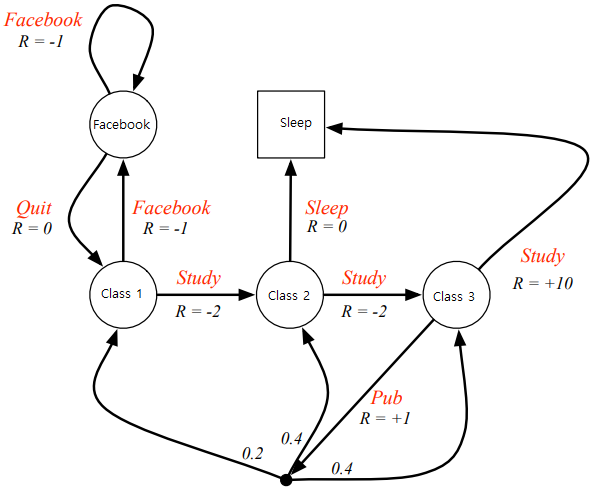
\includegraphics[width=0.33\textwidth]{Figures/MDP.png}
  \end{center}
  \caption{An example of a Markov Decision Process (MDP) for which we might want to learn a specification. (\href{https://medium.com/@bibekchaudhary/markov-decision-process-mdp-simplified-1ae44cf53cc1}{source})}
  \label{fig: mdp}
  \vspace{-0.3cm}
\end{wrapfigure}

To bring us closer to provably safe, interpretable decision-making algorithms for autonomous systems, one approach I am investigating in my research is using machine learning to learn high-level human goals from demonstrations in a way that is amenable to formal control synthesis. Autonomous vehicles exemplify an industry that currently faces many challenges in the field of decision making and control for a safety-critical system. In his annual review in 2018, Schwarting outlined the progress made in the Verification and Synthesis of decision-making and motion planning algorithms \cite{doi:10.1146/annurev-control-060117-105157}. Black box methods (i.e. DNN representing policy / value networks in Deep Reinforcement Learning) are struggling to be verified \cite{doi:10.1146/annurev-control-060117-105157}, which makes their use questionable in such a safety-critical environment. It was particularly noted that while formal control synthesis was of great interest, it does not see wide-spread use cause due to its expensive and the due to the difficulty in formally specifying desired system behavior.

More specifically, my current research consists of first using probabilistic state-machine learning algorithms (e.g. ALERGIA, MDI \cite{prob_state_merging_book}, or RTI(+) \cite{Verwer_PAutomaC}) to learn a probabilistic automaton model representing a human demonstrator's specification for the autonomous system's task. This learning process is based on observed symbol (a symbol is a label for a set of states) sequences (traces) representing system behavior. See Fig. \ref{fig: driving_pdfa_spec} for an example of such a specification. These probabilistic state machines allow are generative in nature, and when sampled from produce traces in the "language" of the probabilistic automaton. This format for the learned specification is more useful than other generative language model (i.e. HMMs or Neural Networks) in one sense, as we can use tools from formal methods to create a controller for the autonomous system we got demonstrations of. Basically, if we can learn the specification for the demonstrator's goals as a state machine, we can compose this specification with a model for the autonomous system's dynamics (e.g. \href{https://en.wikipedia.org/wiki/Transition_system}{transition system} or \href{https://en.wikipedia.org/wiki/Markov_decision_process}{(PO)MDP} -- see Fig. \ref{fig: mdp}) to obtain a correct-by-construction policy to control the system model to follow the learned specification.

\begin{figure}
    \centering
    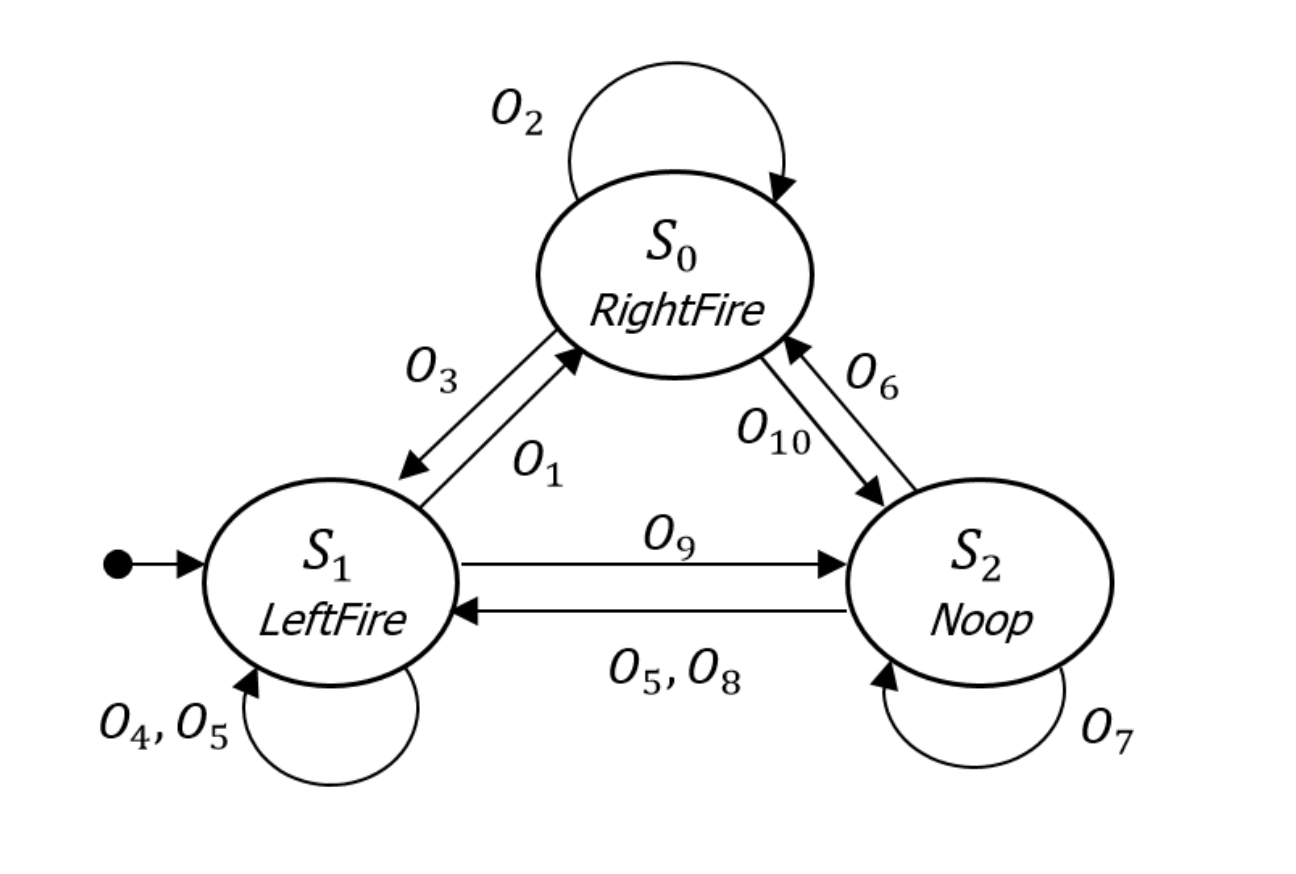
\includegraphics[width=0.4\linewidth]{Figures/pong_moore_machine.png}
    \caption{An example of a three-state moore machine representing an optimal policy for pong for, given a CNN feature extractor that can output observations $O_i$.}
    \label{fig: pong_moore_machine}
\end{figure}

For this project, I would like to focus on tackling both the \textbf{specification learning and synthesis} aspects of the project. The whole goal of learning a specification as an automaton is so we can generate a safe controller for the system from a model of the system and user demonstrations. What is instead all you had was a system to interact with and you wanted to learn an explainable, verifiable controller for the system? Thus, I think it would be very interesting to investigate deep reinforcement learning, as this is the exact sort of machine learning paradigm that would solve such a scenario. Using deep RL but in such a way as to learn a state-machine representation of the eventual policy is of interest to researchers working on explainable AI (XAI) as well as researchers like me working on formal control synthesis for uncertain sequential decision-making systems.